%Dave's handout 1.7 intro 2nd derivatives
%Dave's handout 2.2 2nd derivative rule
\vspace{-0.25 in}
\begin{framed}
\subsection*{Objectives}
\begin{itemize}
    \item Apply the \textbf{Chain Rule} and the product/quotient rules correctly in combination when both are necessary.
    \item Be able to apply the concept of the \emph{Chain Rule} to \textbf{related rates} application.
\end{itemize}

%%%Reading Assignment%%%
\subsection*{Suggested Reading:}
\begin{itemize}
\item \cite{openstax}\footnotemark[1]\textsuperscript{,}\footnotemark[2]
    \begin{itemize}
        \item Section 3.6 The Chain Rule

    \end{itemize}
\item \cite{Calaway}\footnotemark[3]
   \begin{itemize}
         \item Section 2.11 Implicit Differentiation and Related Rates
        \begin{itemize}
            \item Only Examples 3-4.
        \end{itemize}
        
    \end{itemize}


\end{itemize}
%\subsection*{Supplemental Materials:}
%%%Key Terms%%%
\subsection*{Key Terms and Concepts:} 

\begin{multicols}{2}
\begin{itemize}
    \item The Chain and Power Rules combined
    \item The Chain and Product Rules combined
    \item The Chain and Quotient Rules combined
    \item Related Rates
\end{itemize}
\end{multicols}
\end{framed}
\footnotetext[1]{Available free to download from \url{https://openstax.org/details/books/calculus-volume-1} .}
\footnotetext[2]{Disregard any examples with trigonometry.}
\footnotetext[3]{Available free to download from \url{http://www.opentextbookstore.com/details.php?id=14} .}


\newpage
%%%%%%%%%%START LESSON CONTENT%%%%%%%%%%%%%
%\noindent\makebox[\linewidth]{\rule{\textwidth}{0.8pt}}
\Opensolutionfile{ans}[ans11]
\Opensolutionfile{ansL}[ansL11]

\noindent We have seen that for quantities that are changing over time, the rates at which these quantities change are given by derivatives. If two related quantities are changing over time, the rates at which the quantities change are related. For example, if a balloon is being filled with air, both the radius of the balloon and the volume of the balloon are increasing. In lesson \ref{implicitDiff} ,  we consider several variables or quantities are related to each other and some of the variables are changing at a known rate. Then, we study how to determine the relationship between the rates of change of these quantities by using derivatives to determine how rapidly the other variables must be changing.

\subsection*{Application Using The Chain Rule: Related Rates}
%%%From the "Related Rates" box in Applied Calculus by Calaway;Chapter 2 section 11 Implicit Differentiation and Related Rates%%%
\begin{tcolorbox}[title = {Strategy for Finding Related Rates}]
When working with a related rates problem,
\begin{enumerate}
    \item Identify the quantities that are changing, and assign them variables.
    \item Find an equation that relates those quantities.
    \item Differentiate both sides of that equation with respect to time.
    \item Plug in any known values for the variables or rates of change.
    \item Solve for the desired rate.
\end{enumerate}
\end{tcolorbox}

%%Example from Dave's handout 'Implicit Differentiation and Related Rates'

\begin{example}
Suppose the $x$ and $y$ are functions of another variable $t$, and $x$ and $y$ are related by the equation $y^2=4+xy$. Use implicit differentiation with respect to $t$ to determine $\dfrac{dy}{dt}$ in terms of $x,y,$ and $\dfrac{dx}{dt}$.
\vspace*{\stretch{1}}
    %%short answer
    \begin{sol}
    $\dfrac{dy}{dt}=\dfrac{y}{2y-x}\cdot \dfrac{dx}{dt}$
    \end{sol}
    %%solution
    \begin{solL}
    Complete solution here.....
    
    \end{solL}
    
\end{example}


\newpage

%%Example from Dave's handout 'Implicit Differentiation and Related Rates'

\begin{example}
The volume, $V$, of a spherical cancer tumor is given by $V=\dfrac{1}{6}\pi x^3$, where $x$ is the diameter of the tumor.  A physician estimates that the diameter is growing at the rate of 0.4 millimeters per day at the time when the diameter is $x=10$ mm. (NOTE that both $x$ and $V$ are changing with respect to time, $t$.)  Determine the \textbf{rate} at which the volume of the tumor is changing at this point in time.
\vspace*{\stretch{1}}
    %%short answer
    \begin{sol}
    $20\pi$ $mm^3$ per day
    \end{sol}
    %%solution
    \begin{solL}
    Complete solution here.....
    
    \end{solL}
    
\end{example}

%Example 4 from https://openstax.org/books/calculus-volume-1/pages/4-1-related-rates
\begin{example}
A spherical balloon is being filled with air at the constant rate of 2 $cm^3/sec$. How fast is the radius increasing when the radius is 3 cm.?

\begin{figure}[h!]
    \centering
    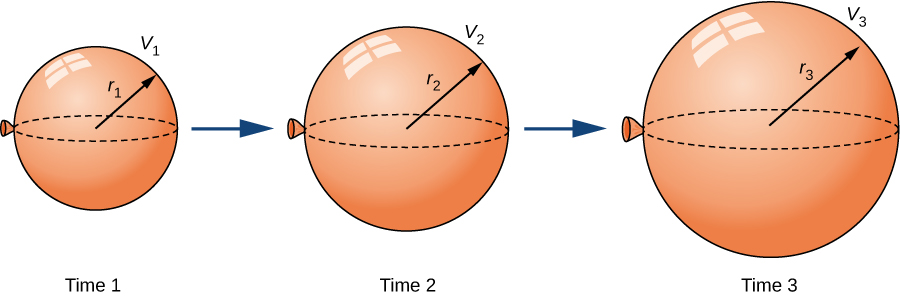
\includegraphics[width=0.7\textwidth]{images/implicitDiff/ballon.jpg}
\end{figure}
    %%short answer
    \begin{sol}
    $\dfrac{1}{18\pi}$ cm. per second
    \end{sol}
    %%solution
    \begin{solL}
    Complete solution here.....
    
    \end{solL}
    
\end{example}
\vspace*{\stretch{1}}
\newpage
%%Example from https://youtu.be/ZAgFwsOxSgU%%%

\begin{wrapfigure}[7]{r}{0.35\textwidth}
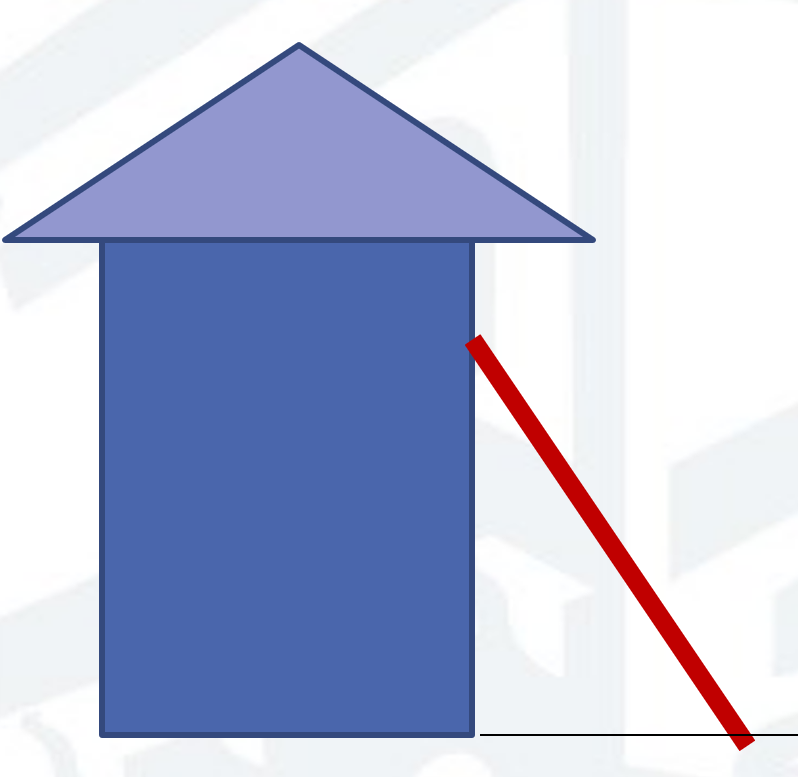
\includegraphics[width=0.7\textwidth]{images/implicitDiff/houseLadder.PNG}
\end{wrapfigure}
\hfill \break
\vspace{-0.5in}
\begin{example}
A 12 foot ladder is leaning up against a house. The base of the ladder begins to slip away from the house at a rate of 0.5 ft per second. How fast is the top of the ladder moving down the side of the house when the ladder 3 feet away from the house?\\
\url{https://www.geogebra.org/m/xnuumrcf}
\vspace*{\stretch{1}}
    %%short answer
    \begin{sol}
    $-0.13$ ft. per second
    \end{sol}
    %%solution
    \begin{solL}
    Complete solution here.....
    
    \end{solL}
    
\end{example}
\newpage
%%%Example 3 from Applied Calculus by Calaway;Chapter 2 section 11 Implicit Differentiation and Related Rates%%%

\begin{wrapfigure}[7]{r}{0.35\textwidth}
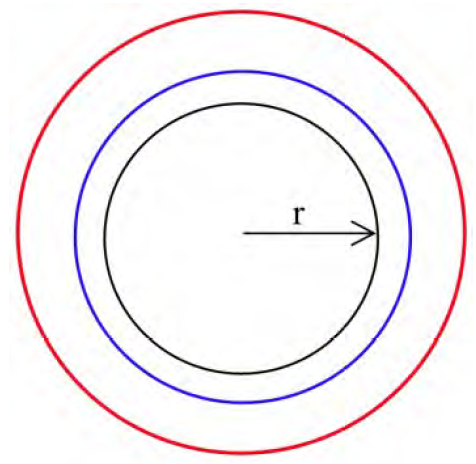
\includegraphics[width=0.7\textwidth]{chainRule/exTownBorder.png}
\end{wrapfigure}
\hfill \break
\vspace{-0.5in}
\begin{example}
Suppose the border of a town is roughly circular, and the radius of that circle has been increasing at a rate of 0.1 miles each year. 
\renewcommand{\labelenumi}{\textbf{(\alph{enumi})}}
\begin{enumerate}[leftmargin=*]
    \item Determine the equation that gives the relationship between the \textbf{town area} (in mile\raise0.75ex\hbox{\scriptsize{2}}) , $\bm{A}$ and the town radius (in mile), $\bm{r}$. \emph{Include the appropriate unit.} \vspace*{\stretch{1.5}}
\end{enumerate}

\renewcommand{\labelenumi}{\textbf{(\alph{enumi})}}
\begin{enumerate}[leftmargin=*]
    \setcounter{enumi}{1}
    \item Determine the equation that gives the relationship between the \textbf{town radius} , $\bm{r}$ and the time (in year), $\bm{t}$. That is, find the value of $\frac{dx}{dt}$. \emph{Include the appropriate unit.}\vspace*{\stretch{1}}
    \item Using the \textbf{Chain Rule}, determine the \textbf{related rates equation} that gives the relationship between the rate of change of the town area, $\displaystyle\frac{dA}{dt}$ and the rate of change of the town radius, $\displaystyle\frac{dr}{dt}$. \emph{Include the appropriate unit.}\vspace*{\stretch{4}}
    \item Find \textbf{how fast the area} of the town has been increasing when the radius is 5 miles. \emph{Include the appropriate unit.} \vspace*{\stretch{1}}
    
\end{enumerate}
    %%short answer
    \begin{sol}
    \onehalfspacing{
    \begin{enumInline1}
    \item $A(r)=\pi r^2$ mile\raise0.75ex\hbox{\scriptsize{2}} 
    \item $r(t)=0.1t$ mile per year
    \item $\displaystyle\frac{dA}{dt}=2\pi r\displaystyle\frac{dr}{dt}$ mile\raise0.75ex\hbox{\scriptsize{2}}
    \item Around 3.14 mile\raise0.75ex\hbox{\scriptsize{2}} per year
    \end{enumInline1} }
    \end{sol}
    %%solution
    \begin{solL}
    Complete solution here.....
    
    \end{solL}
    
\end{example}
\newpage
%%%%%%%%%Example 4 from Calaway; Applied Calculus; 2.11 Implicit Differentiation and Related Rates%%%%%%%%%%
\begin{example}
A company has determined the demand curve for their product is
\begin{equation*}
q=\sqrt{5000-p^2}
\end{equation*}

\noindent where $p$ is the price in dollars, and $q$ is the quantity in millions. The quantities changing are $p$ and $q$, and we assume they are both functions of time, $t$, in weeks. We already have an equation relating the quantities.\\

\noindent If weather conditions are driving the price up \$2 a week, find \textbf{the rate at which demand is changing when the price is \$40}. Include the appropriate units. Interpret the result.
    %%short answer
    \begin{sol}
    $-1.37$ million items per week ; Demand is \underline{falling} by 1.37 million items per week.
    \end{sol}
    %%solution
    \begin{solL}
    Complete solution here.....
    
    \end{solL}
    
\end{example}
\vspace*{\stretch{1}}
%%%%%%%%%%%%%%%End Lesson%%%%%%%%%%%%%%%%%%
\Closesolutionfile{ans}
\Closesolutionfile{ansL}

%%%Short Answers to Examples%%%
\vspace*{\fill}

\subsection*{Short Answers to Examples}
%\vspace{-0.25cm}
%\begin{multicols}{2}
\input{ans11}
%\end{multicols}


